\begin{table}[h!]
	\centering
	\caption{Random Forest Hyperparameters}
	\begin{tabular}{ll}
		\hline
		\textbf{Parameter} & \textbf{Value} \\
		\hline
		n\_estimators & 1000 \\
		random\_state & 42 \\
		class\_weight & balanced \\
		min\_samples\_leaf & 5 \\
		min\_samples\_split & 10 \\
		\hline
	\end{tabular}
\end{table}

\begin{table}[h!]
	\centering
	\caption{Random Forest Classification Performance}
	\begin{tabular}{lcccc}
		\hline
		\textbf{Class} & \textbf{Precision} & \textbf{Recall} & \textbf{F1} & \textbf{Support} \\
		\hline
		Normal (0) & 1.00 & 0.99 & 0.99 & 15411 \\
		Attack (1) & 0.98 & 1.00 & 0.99 & 14293 \\
		\hline
		\textbf{Accuracy} & \multicolumn{4}{c}{0.9922} \\
		Macro Avg & 0.99 & 0.99 & 0.99 & 29704 \\
		Weighted Avg & 0.99 & 0.99 & 0.99 & 29704 \\
		\hline
	\end{tabular}
\end{table}

\begin{table}[h!]
	\centering
	\caption{Training and Test Set Class Distribution}
	\begin{tabular}{lcc}
		\hline
		\textbf{Class} & \textbf{Train Count} & \textbf{Test Count} \\
		\hline
		Normal (0) & 61643 & 15411 \\
		Attack (1) & 57170 & 14293 \\
		\hline
	\end{tabular}
\end{table}


\begin{figure}[h!]
	\centering
	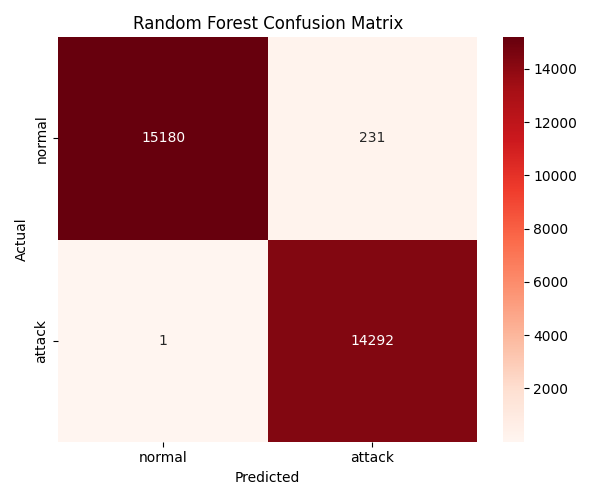
\includegraphics[width=0.45\textwidth]{rf_confusion_matrix-1000-5-42-True.png}
	\caption{Confusion matrix for the Random Forest model (1000 estimators, min\_samples\_leaf = 5, random\_state = 42, datasets combined).}
	\label{fig:rf_confusion_matrix_1}
\end{figure}
